\documentclass[markcolor=black,trimmed,coverwidth=6in,coverheight=9in,bleedwidth=0.0in,spinewidth=0.4in,11pt]{bookcover}
\usepackage[utf8]{inputenc}
\usepackage[T1]{fontenc}
\usepackage[english]{babel}
\usepackage{garamondx}
\usepackage{microtype}
\usepackage{adforn}
\definecolor{ceruleanblue}{HTML}{9BC4E2}

\colorlet{title}{ceruleanblue}
\colorlet{spinebg}{ceruleanblue}
\colorlet{body}{black}

\begin{document}
\begin{bookcover}
\bookcovercomponent{color}{bg front}{color=black}
\bookcovercomponent{color}{bg back and spine}{color=spinebg}

\bookcovercomponent{tikz}{bg spine}{
\node (rect) at ([yshift=1.05878871572302229236\coverwidth]part.south east) {};
\fill[black] (part.north west) rectangle (rect);
\fill[spinebg] (part.south west) rectangle (rect);
}

\bookcovercomponent{center}{spine}{
    \rotatebox[origin=c]{-90}{\textbf{{\color{title} COLLECTED POEMS} \qquad {\color{body}Alice Moore}} \hspace{4.5in}}}


\bookcovercomponent{normal}{front}{
\vspace{4\baselineskip}
\begin{center}
\color{title}
{\Huge \textbf{COLLECTED POEMS}}\\
\vspace{2\baselineskip}
{\LARGE Alice Moore}
\end{center}
\vfill
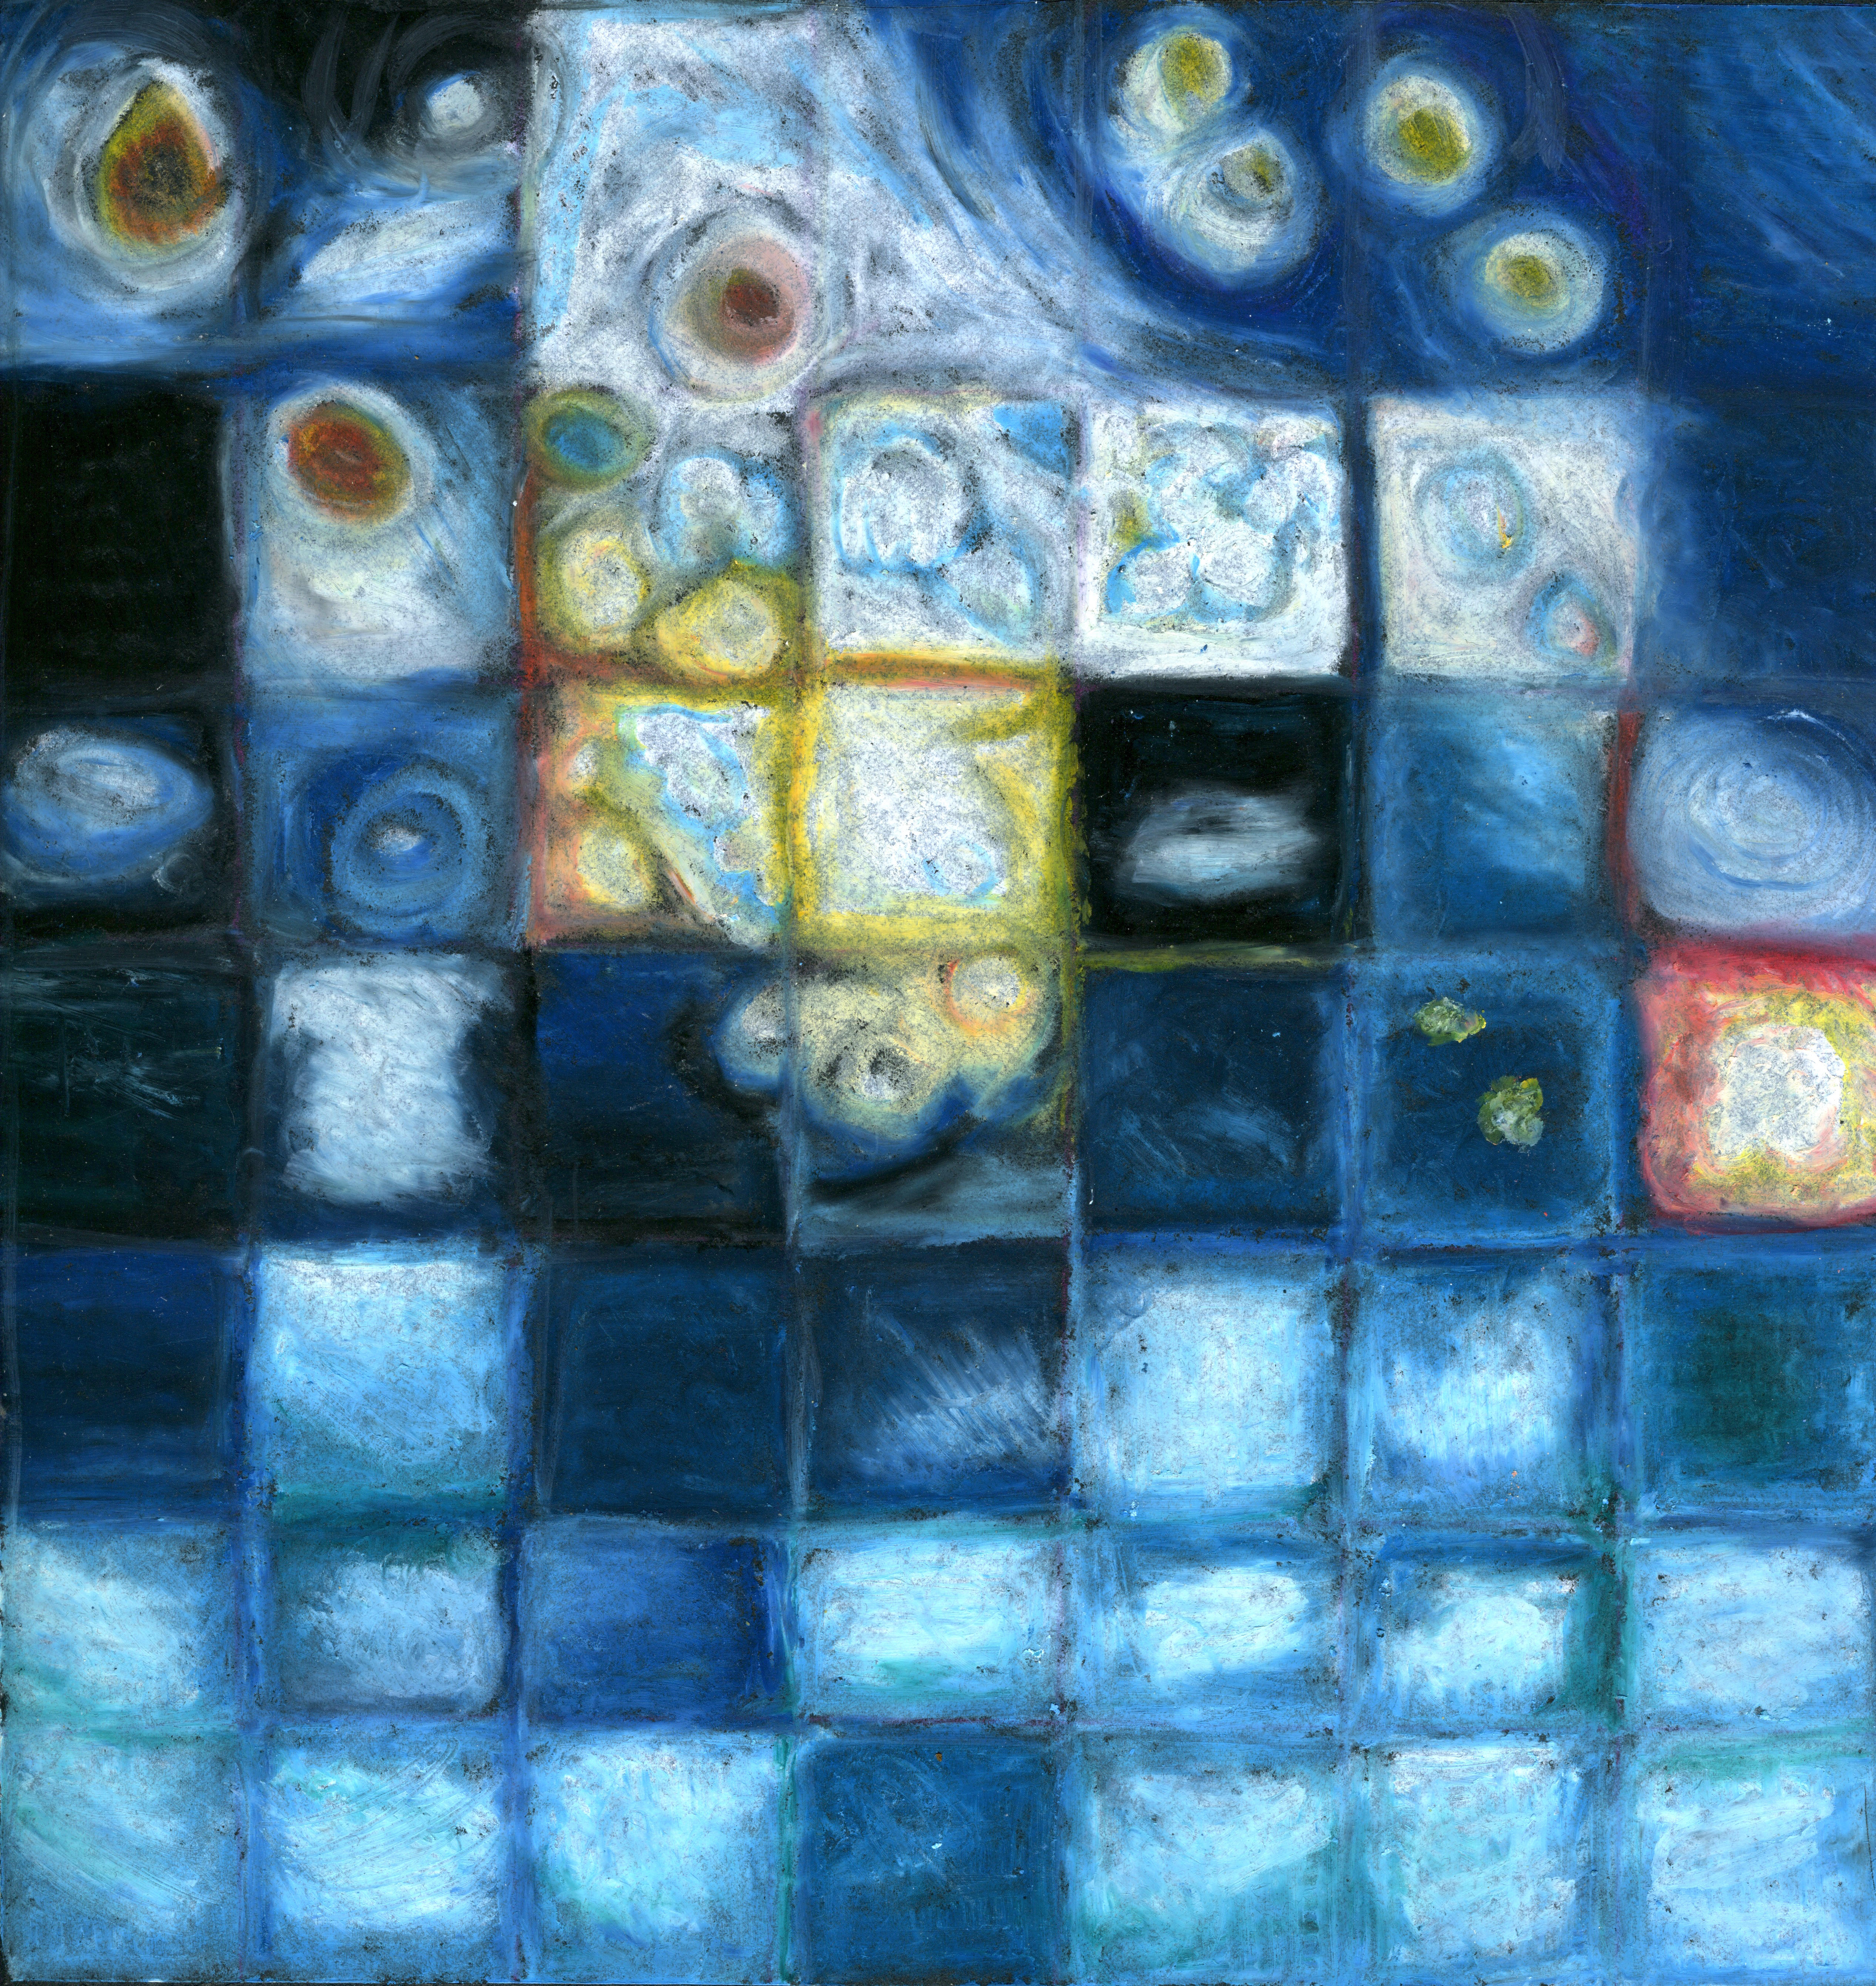
\includegraphics[width=\coverwidth]{./painting}
}

\bookcovercomponent{normal}{back}{
\vspace{3\baselineskip}
\begin{center}
\includegraphics[width=4.5in]{./alice_dusty}
\par\vspace{1\baselineskip}
\parbox{4.5in}{\color{body} Alice Moore was born on April 23, 1952, in Providence, Rhode Island. She taught for many years as an Associate Professor in the Humanities at Corning Community College. Alice passed away at home in Candor, New York on April 28, 2017, and is survived by her partner Tom Cole and sons Alex and Will.}
\end{center}
}

\end{bookcover}
\end{document}